\section{Physikalische Grundlagen}
Die Ausführungen dieses Kapitels basieren auf \cite{manual}.
\subsection{Kernspin}
\subsubsection{Definition}
Der mechanische Drehimpuls eines Atomkerns, verursacht durch die Eigenrotation um den Schwerpunkt, wird \emph{Kernspin} $\vec{I}$
genannt. Er folgt den Gesetzten eines quantenmechanischen Drehimpulses: Nur sein Betrag $|\vec{I}|$ und die Projektion $I_z$ auf 
eine \emph{Quantisierungachse}, welche frei wählbar ist und meistens parallel zur $z$-Achse gelegt wird, können gleichzeitig 
bestimmt werden. Für den Betrag $|\vec{I}|$ gilt:
\begin{equation}
  \label{eq:spin:abs}
  |\vec{I}| = \hbar \sqrt{I (I + 1)}
\end{equation}
mit der \emph{Kernspinquantenzahl} $I \geq 0$. Die Projektion $I_z$ auf die $z$-Achse ergibt sich zu
\begin{equation}
  \label{eq:spin:z}
  I_z = m_I \cdot \hbar .
\end{equation}
Die \emph{magnetische Kernspinquantenzahl} $m_I$ kann dabei nur $2 I + 1$ entweder ganz- oder halbzahlige Werte im Bereich von 
$-I \geq m_I \geq I$ annehmen.
\subsubsection{Verschiedene Beispiele für $I$}
Protonen und Neutronen besitzen einen Kernspin von $I=\frac{1}{2}$, daher kann $m_I$ nur die Werte $\pm\frac{1}{2}\hbar$ annehmen. \\
Bei Atomkernen werden alle Kernspins der Nukleonen aufaddiert. Hierzu wird die g-u-Nomenklatur eingeführt: Eine gerade Anzahl von 
Protonen oder Neutronen wird mit \emph{g} bezeichnet, eine Ungerade mit \emph{u}. Jeder Kern besitzt zwei dieser Zustände, sie werden hintereinander 
aufgelistet (\emph{gg}, \emph{uu}, \emph{gu}, \emph{ug}), dabei bezeichnet der erste Buchstaben die Anzahl der Protonen, der Zweite die der 
Neutronen.\\
Im Grundzustand folgen die Nukleonen dem Pauliprinzip, da sowohl Protonen als auch Neutronen aus Fermionen aufgebaut sind. 
Ein Orbital wird mit zwei Protonen oder Neutronen, deren Kernspin in gegensätzliche  
Richtungen zeigt, gefüllt. Daher haben \emph{gg}-Kerne einen Kernspin von $I = 0$. Für \emph{gu}- und \emph{ug}-Kerne gilt $I = \frac{1}{2}$. 
Bei \emph{uu}-Kernen gilt $I=1$, da das Pauliprinzip nur für Teilchen gleicher Art gilt.

\subsection{Magnetisches Moment}
Durch den Kernspin $\vec{I}$ folgt ein \emph{magnetischen Dipolmoment} $\vec{\mu}$:
\begin{equation}
  \label{eq:mu:vec}
  \vec{\mu} = \gamma \cdot \vec{I}
\end{equation}
Dabei ist die Proportionalitätskonstante $\gamma$ das \emph{gyromagnetische Verhältnis}:
\begin{equation}
  \label{eq:gamma}
  \gamma = \frac{g_I \cdot \mu_K}{\hbar}
\end{equation}
Hier ist $g_I$ der \emph{Kern-g-Faktor}, eine kernspezifische Größe, und $\mu_K$ das Kernmagneton (analog zum Bohrschen Magneton, nur mit der 
Protonenmasse $m_P$ anstatt der Elektronenmasse):
\begin{equation}
  \label{eq:muK}
  \mu_K = \frac{e \cdot \hbar}{2 m_P}
\end{equation}
Mit \autoref{eq:spin:z} und \autoref{eq:gamma} folgt für die $z$-Komponente des magnetischen Dipolmoments aus \autoref{eq:mu:vec}:
\begin{equation}
  \label{eq:mu:z}
  \mu_z = g_I \cdot \mu_K \cdot m_I
\end{equation}

\subsection{Kernspinresonanz}
\subsubsection{Der Kern im äußeren Magnetfeld}
Legt man an das Atom ein äußeres Magnetfeld $\vec{B}$ an, so besitzt der Kern mit dem magnetischen Dipolmoment $\mu$ folgende Energie:
\begin{equation}
  E = - \vec{\mu} \cdot \vec{B}
\end{equation}
Für ein Magnetfeld in $z$-Richtung ($\vec{B} = B \cdot \hat{e}_z$) folgt mit \autoref{eq:mu:z}:
\begin{equation}
  E = - g_I \cdot \mu_K \cdot m_I \cdot B
\end{equation}
Es entstehen folglich mehrere energetische Niveaus, die von $m_I$ abhängen. Die Differenz $\Delta E$ zwischen zwei benachbarten Niveaus 
(Zeemanaufspaltung) beträgt, da $\Delta m_I = \pm 1$:
\begin{equation}
  \label{eq:deltaE}
  \Delta E = g_I \cdot \mu_K \cdot B
\end{equation}

\subsubsection{Wechselwirkung mit einem Strahlungsfeld}
Der Kern kann zwischen den verschiedenen Energieniveaus (Zuständen) durch spontane oder induzierte Emission und Absorption von Photonen übergehen. 
Die Photonen (aus einem Strahlungsfeld) müssen für solch einen Übergang nach \autoref{eq:deltaE} eine ganz bestimmte Energie besitzten, man spricht 
von \emph{Resonanz}. Für die \emph{Resonanzfrequenz} gilt nun:
\begin{equation}
  \label{eq:nu}
  \nu = \frac{\Delta E}{h} \refeq{eq:deltaE} \frac{g_I \cdot \mu_K \cdot B}{h} \refeq{eq:gamma} \frac{\gamma \cdot B}{2 \pi}
\end{equation}
Experimentell lässt sich diese Resonanzfrequenz nur mit einer endlichen Linienbreite bestimmen. Gründe dafür sind Effekte wie die natürliche 
Linienbreite (Energie-Zeit-Unschärfe), der Dopplereffekt und Stöße.

\subsubsection{Besetzungszahlen}
In diesem Versuch haben alle zu untersuchenden Atome und Moleküle einen Kernspin von $I=\frac{1}{2}$, also $m_I = \pm \frac{1}{2}$. Es ergeben sich 
folglich zwei verschiedene Energieniveaus ($E_{\text{hoch}}$ und $E_{\text{tief}}$, $E_{\text{hoch}} > E_{\text{tief}}$) mit den 
Besetzungszahlen $n_{\text{hoch}}$ und $n_{\text{Anzahl}}$. 
Diese liegen im thermischen Gleichgewicht unter der Boltzmannverteilung vor. Für das Verhältnis der beiden Besetzungszahlen gilt:
\begin{equation}
  \frac{n_{hoch}}{n_{tief}} = e^{-\frac{E_\text{hoch} - E_\text{tief}}{k \cdot T}} = e^{- \frac{\Delta E}{k \cdot T}} > 0
\end{equation}
Das tiefere Energieniveau ist also mehr besetzt als das Höhere. Daher werden mehr Photonen des Strahlungsfeldes absorbiert als neue Photonen durch 
Emission gewonnen werden, das Strahlungsfeld verliert an Energie. Dieser Effekt kann durch die Dämpfung des Schwingkreises, welcher das 
Strahlungsfeld erzeugt, gemessen werden.

\subsubsection{Relaxationsprozesse}
Über einen längeren Zeitraum betrachtet sollten sich die Besetzungszahlen der beiden Energieniveaus annähern, was zu einer Reduktion des oben 
beschriebenen Effekts führt. Dieser Abnahme wird durch \emph{Relaxationsprozesse} entgegengewirkt, durch welche die höherenergetischen Zustände 
in die niederenergetischen Zustände zurückfallen, ohne dabei Strahlung abgeben. \\
Wird die Energie bei dieser Zustandsänderung in Form von Wärme an das Gitter des Materials ab, so spricht man von \emph{Spin-Gitter-Relaxation}. \\
Des Weiteren gibt es die \emph{Spin-Spin-Relaxation}. %TODO Erklärung.

\subsection{Der Hall-Effekt}
Bringt man einen stromdurchflossenen Leiter in ein Magnetfeld,
dann wirkt auf die Leitungselektronen die Lorentzkraft $\vec{F_L}$:
\begin{equation}
\label{eq:lorentz}
\vec{F_L} = q \cdot (\vec{v} \times \vec{B})
\end{equation}
Die Elementarladung ist $q$, $\vec{v}$ die Driftgeschwindigkeit der Elektronen und $\vec{B}$ das Magnetfeld.
Durch die Kraft werden die Elektronen gegenüber den festen Atomrümpfen verschoben und es
bildet sich ein elektrisches Feld $\vec{E}$ aus,
das auf die Elektronen die Kraft
\begin{equation}
\label{eq:Fe}
\vec{F_C} = \vec{E} \cdot q
\end{equation}
ausübt. Mit
\begin{equation}
\label{}
 U_H = \frac{E}{d},
\end{equation}
dem Kräftegleichgewicht $\vec{F_L} = \vec{F_C}$ und $\vec{v} \perp \vec{B}$ folgt
\begin{equation}
  U_H = v \cdot B \cdot d \ \, .
\end{equation}
Es bildet sich also eine Hall-Spannung $U_H$ aus, die proportional zur Stärke des Magnetfelds ist und
als Messsignal verwendet werden kann.
\autoref{img:hall} zeigt diese Verhältnisse am Leiter.

\begin{figure}[H]
\begin{center}
  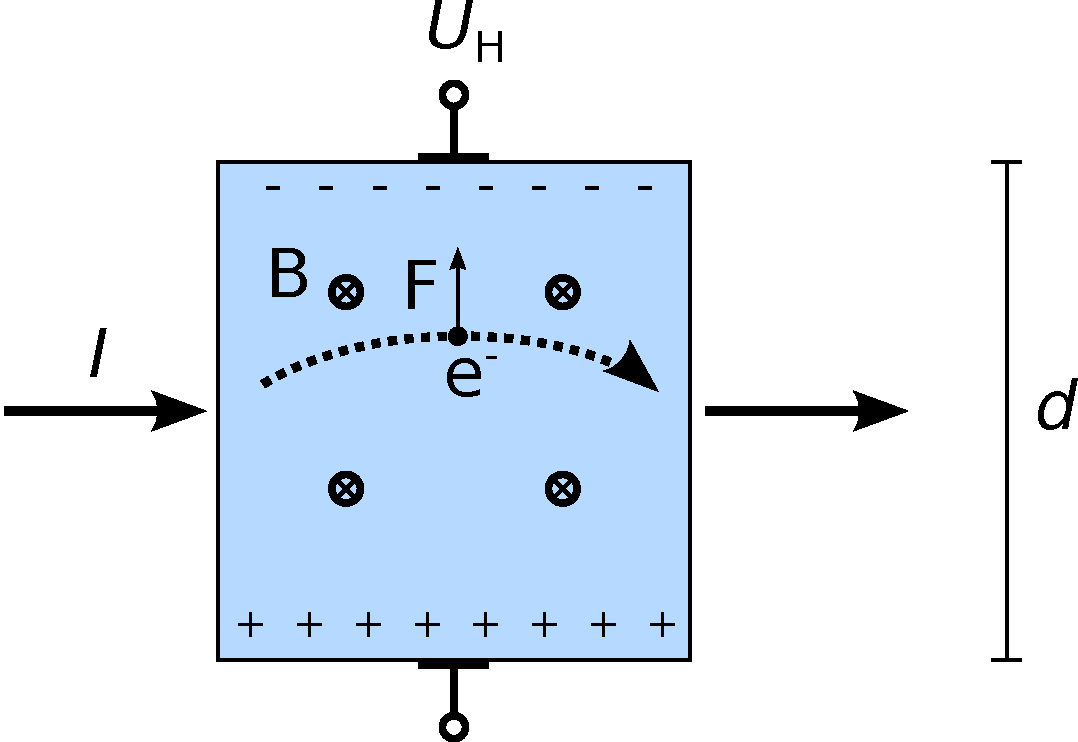
\includegraphics[width=0.5\textwidth]{../img/hall.pdf}
  \caption{Hall-Effekt: Ablenkung von bewegten Elektronen im Leiter.}
  \label{img:hall}
\end{center}
\end{figure}